\documentclass[11pt,aspectratio=169]{beamer}

\usepackage{fontspec}
\usepackage{graphicx}
\usepackage{booktabs}
\usepackage{array}
\usepackage{xcolor}
\usepackage{amsmath}
\usepackage{appendixnumberbeamer}

\setmainfont{DejaVu Serif}
\setsansfont{DejaVu Sans}
\setmonofont{DejaVu Sans Mono}

\usetheme{metropolis}
\metroset{progressbar=frametitle, numbering=fraction, sectionpage=progressbar}

\definecolor{accent}{HTML}{1F6FB2}
\definecolor{warm}{HTML}{C0504D}
\definecolor{soft}{HTML}{4F81BD}
\setbeamercolor{progress bar}{fg=accent}
\setbeamercolor{title separator}{fg=accent}
\setbeamercolor{frametitle}{bg=accent, fg=white}

\graphicspath{{../results/}}

\title{Profiling Vision-Language Models}
\subtitle{Performance, energy, and where the time actually goes}
\author{Vladislav Smirnov}
\institute{Project supervisor: Egor (\texttt{@daLime})}
\date{April 2026}

\begin{document}

\maketitle

% ====================================================================
\begin{frame}{The question}
  \textbf{Project goal:} understand how VLMs scale and where to spend optimization effort.
  \vfill
  Two concrete questions:
  \begin{enumerate}
    \item Which models are Pareto-optimal on quality / latency / energy?
    \item \textbf{Which parts of the model dominate cost?} (the supervisor's main question)
  \end{enumerate}
  \vfill
  Approach: vary one axis at a time, measure four things directly, then split the dominant model into sub-components.
\end{frame}

% ====================================================================
\begin{frame}{Setup}
  \footnotesize
  \begin{columns}[T,onlytextwidth]
    \column{0.55\textwidth}
    \textbf{Models (7)}
    \begin{itemize}\setlength\itemsep{0pt}
      \item \texttt{blip2-opt-2.7b}, \texttt{blip2-flan-t5-xl}
      \item \texttt{instructblip-flan-t5-xl}, \texttt{instructblip-vicuna-7b}
      \item \texttt{llava-1.5-7b}, \texttt{llava-1.5-13b}
      \item \texttt{fuyu-8b}
    \end{itemize}
    \vspace{1mm}
    \textbf{Datasets (300 samples each)}: ScienceQA, TextVQA, COCO Captions

    \column{0.45\textwidth}
    \textbf{Axes varied}
    \begin{itemize}\setlength\itemsep{0pt}
      \item Resolution: 224 / 336 / 448 / 512
      \item Prompt: 10 / 50 / 100 / 200 tokens
      \item Batch: 1 / 2 / 4 / 8
      \item FP32, FP16, \texttt{torch.compile}, FA2
      \item GPU vs.\ CPU
    \end{itemize}
    \vspace{1mm}
    \textbf{Metrics}: latency, FLOPs, energy (J), WER.\\
    \textbf{Hardware}: 2× RTX 5880 Ada, 48 GiB.
  \end{columns}
\end{frame}

% ====================================================================
\begin{frame}{Baseline: two clear tiers}
  \begin{columns}[T,onlytextwidth]
    \column{0.58\textwidth}
    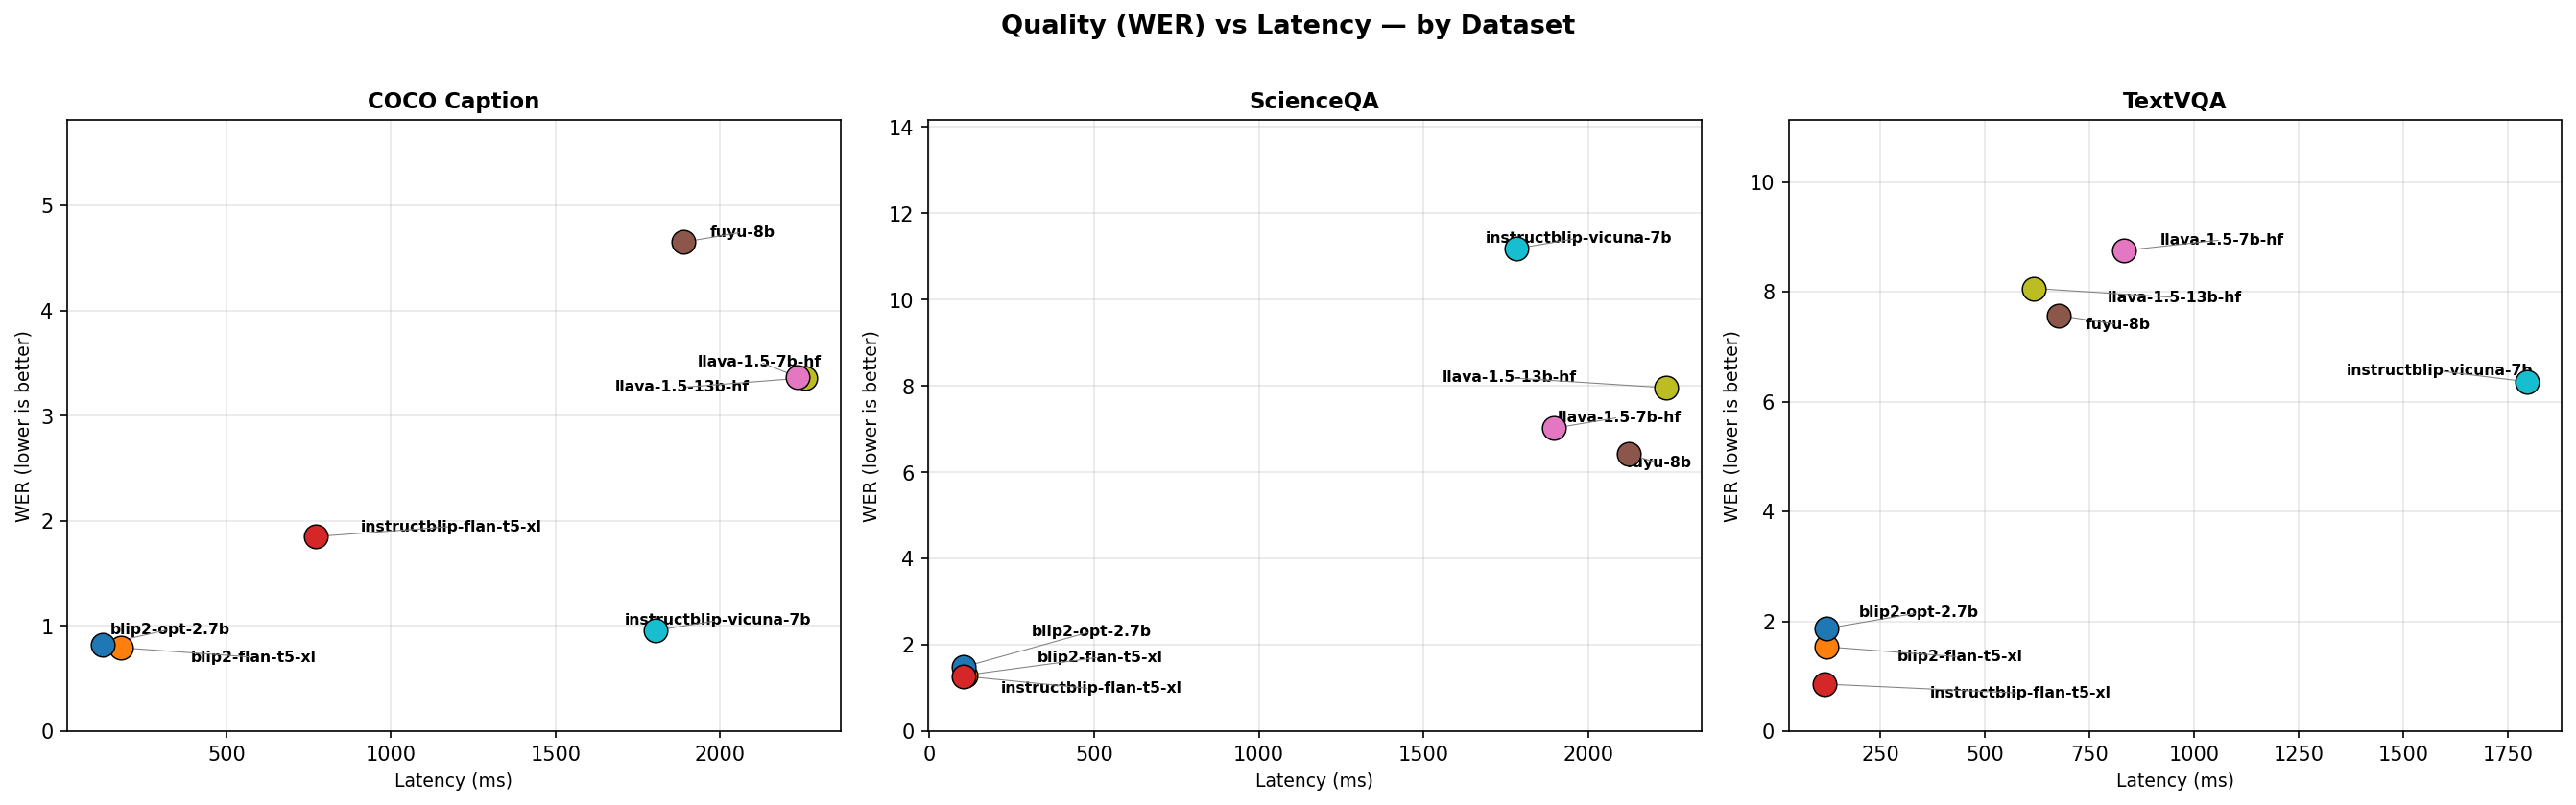
\includegraphics[width=\textwidth]{quality_vs_latency_by_dataset.png}

    \column{0.42\textwidth}
    \scriptsize
    \begin{tabular}{@{}lrr@{}}
      \toprule
      Model & Lat ms & Energy J \\
      \midrule
      blip2-flan-t5-xl        &   136 &  31 \\
      blip2-opt-2.7b          &   115 &  29 \\
      instructblip-t5-xl      &   330 &  70 \\
      \midrule
      fuyu-8b                 & 1\,562 & 404 \\
      llava-1.5-7b            & 1\,654 & 450 \\
      llava-1.5-13b           & 1\,704 & 470 \\
      instructblip-vicuna-7b  & 1\,793 & 487 \\
      \bottomrule
    \end{tabular}
    \vspace{2mm}

    \footnotesize
    \textbf{Pareto winner:} \texttt{blip2-flan-t5-xl} — WER 1.21, 136 ms, 31 J.
    \vspace{1mm}

    7B+ tier: 10–15× slower, 6–15× more energy, marginal quality gain.
  \end{columns}
\end{frame}

% ====================================================================
\begin{frame}{What didn't work, and why}
  \scriptsize
  \begin{tabular}{@{}p{0.28\textwidth}p{0.68\textwidth}@{}}
    \toprule
    \textbf{Attempted} & \textbf{Why it failed / what we did} \\
    \midrule
    \texttt{idefics2-8b} &
      Pixel-values shape mismatch on \texttt{transformers} 5.x (``expected 5, got 4''). Dropped from results. \\
    \texttt{cogagent}, \texttt{moondream2}, \texttt{llava-400m-fp16} &
      Bespoke \texttt{trust\_remote\_code}; last one isn't on HF (likely typo). Used \texttt{llava-1.5-7b} for same-family comparison. \\
    \texttt{torch.compile} on T5 &
      Compiler bails on encoder-decoder graph. No measurable speedup on the others either. \\
    FP16 on T5 &
      \emph{Slower} than FP32 — internal dtype casts inside T5's forward. \\
    FP16 on \texttt{fuyu-8b} &
      Float / Half dtype mismatch in the patch-embedding path. \\
    \texttt{flash-attn} pip & Build needs \texttt{nvcc} $\geq$ 11.7; system has 11.5. Used PyTorch SDPA instead, which dispatches FA2 in FP16 on Ada. \\
    Batched \texttt{fuyu-8b} & Processor returns lists for \texttt{batch>1}; skipped the batch sweep for Fuyu. \\
    \bottomrule
  \end{tabular}
\end{frame}

% ====================================================================
\begin{frame}{The punchline: where the time goes}
  \begin{columns}[T,onlytextwidth]
    \column{0.62\textwidth}
    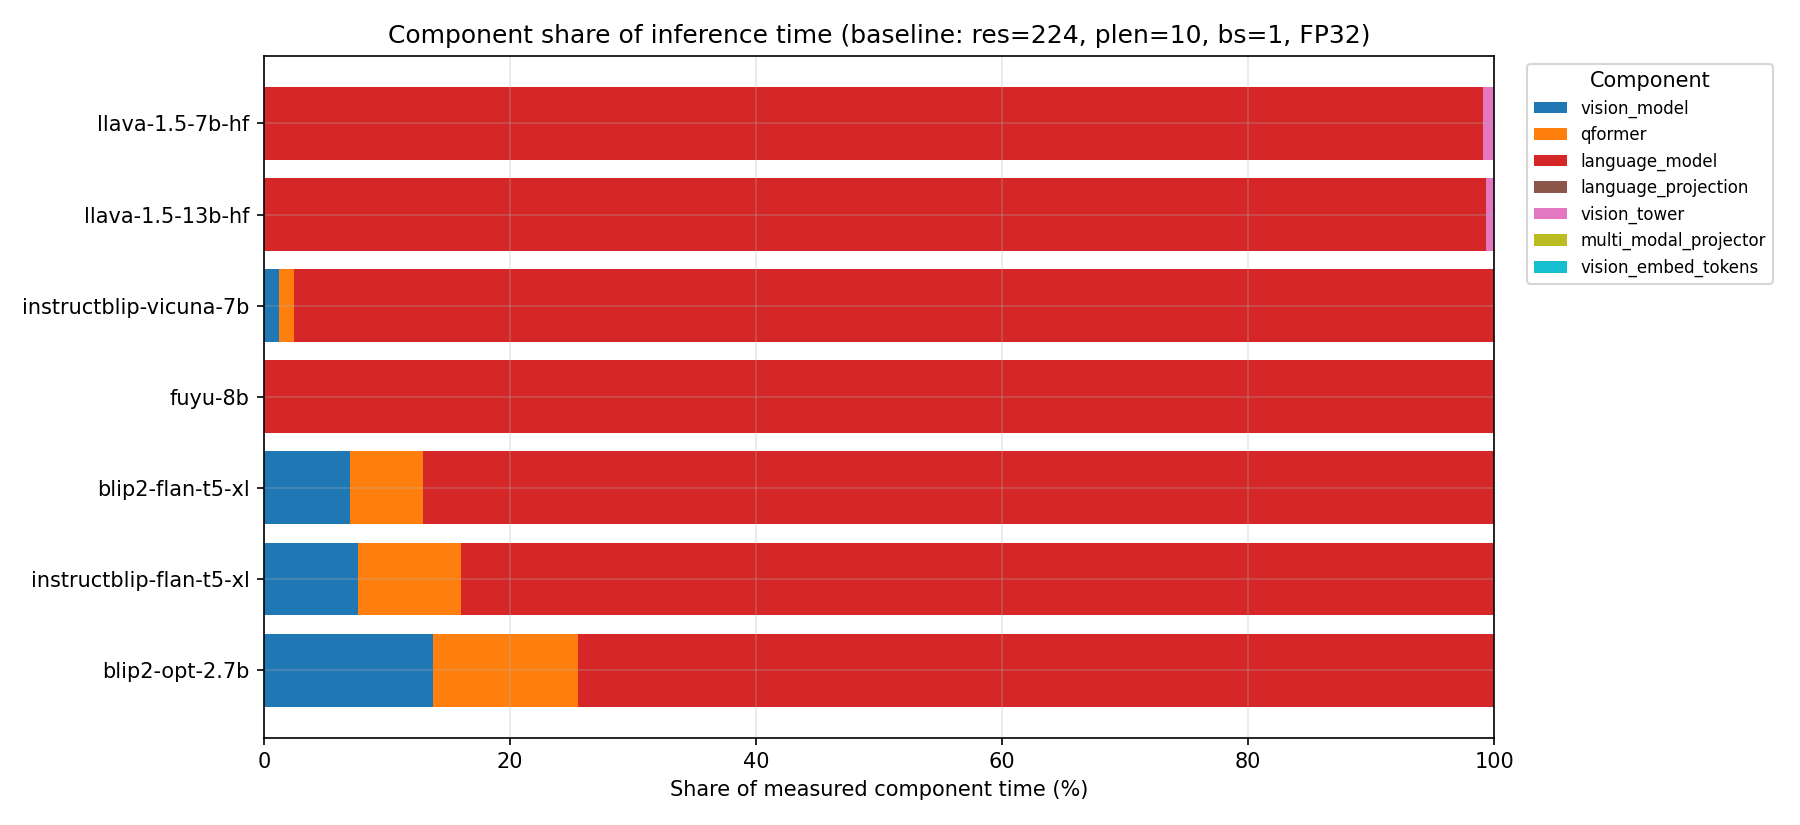
\includegraphics[width=\textwidth]{component_latency_share.png}

    \column{0.38\textwidth}
    \scriptsize
    Forward hooks + CUDA events on top-level submodules.
    \vspace{2mm}

    \textbf{LLM decoder share:}
    \begin{itemize}\setlength\itemsep{0pt}
      \item BLIP-2 OPT 2.7b: \textbf{74\%}
      \item BLIP-2 / InstructBLIP T5: 84–87\%
      \item All 7B+ models: \textbf{98–99.99\%}
    \end{itemize}
    \vspace{2mm}

    Vision encoder is \emph{not} the bottleneck — explains flat latency-vs-resolution.\\[1.5mm]
    \textcolor{accent}{\textbf{Optimize the decoder.}}
  \end{columns}
\end{frame}

% ====================================================================
\begin{frame}{Inside the decoder: prefill vs.\ per-token decode}
  \begin{columns}[T,onlytextwidth]
    \column{0.58\textwidth}
    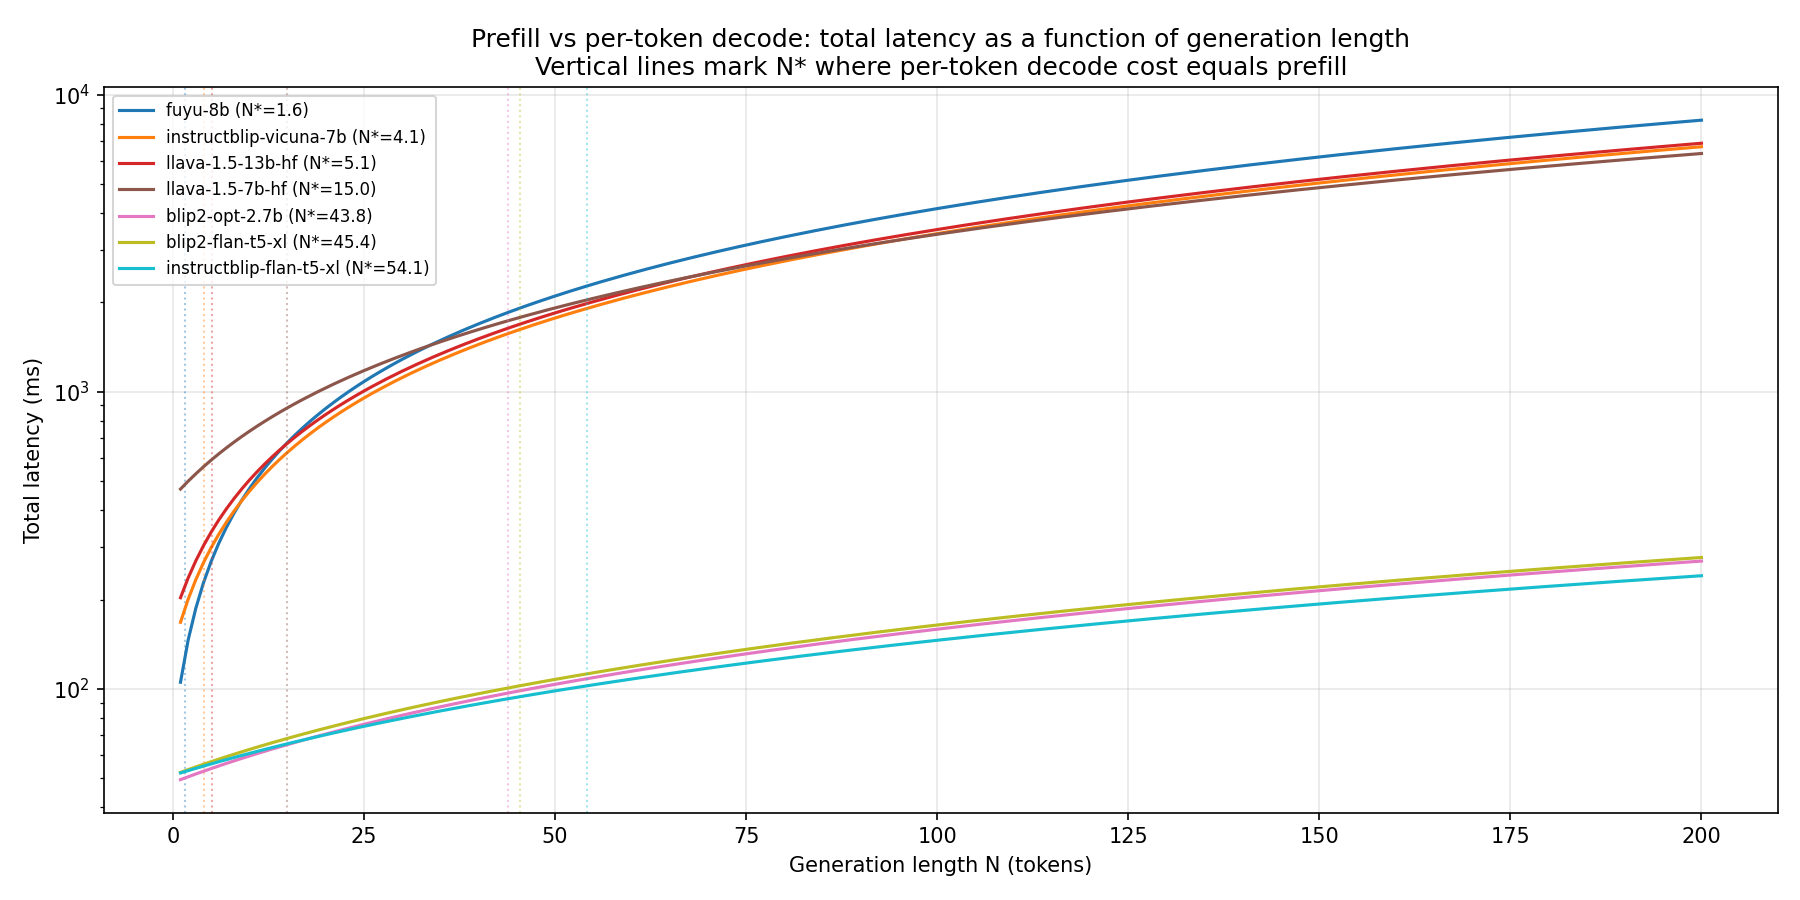
\includegraphics[width=\textwidth]{prefill_decode_crossover.png}

    \column{0.42\textwidth}
    \scriptsize
    Fit $t(N) = t_{\text{prefill}} + N\,t_{\text{decode}}$ from $N{=}1$ and $N{=}50$.
    \vspace{1.5mm}

    \textbf{Crossover} $N^* = t_{\text{prefill}}/t_{\text{decode}}$:
    \begin{itemize}\setlength\itemsep{0pt}
      \item fuyu-8b: 1.6
      \item instructblip-vicuna-7b: 4.1
      \item llava-1.5-13b: 5.1
      \item BLIP-2 family: 44–54
    \end{itemize}
    \vspace{1.5mm}

    \textbf{Lever:}
    \begin{itemize}\setlength\itemsep{0pt}
      \item Short ($\leq 10$ tok): optimize prefill — FA2, chunked prefill
      \item Long ($\geq 50$ tok): optimize decode — speculative, KV-cache quant
    \end{itemize}
  \end{columns}
\end{frame}

% ====================================================================
\begin{frame}{FlashAttention-2: smaller win than expected}
  \footnotesize
  \begin{tabular}{@{}lcccc@{}}
    \toprule
     & SDPA prefill & eager prefill & FA2 speedup & decode/tok (SDPA / eager) \\
    \midrule
    \texttt{llava-1.5-7b}  &  94.5 ms & 105.4 ms & \textbf{1.11×} & 15.3 / 15.6 ms \\
    \texttt{llava-1.5-13b} & 169.0 ms & 181.3 ms & \textbf{1.07×} & 33.0 / 34.2 ms \\
    \bottomrule
  \end{tabular}
  \vspace{3mm}

  \normalsize
  \textbf{Why so modest?} At plen=10 the LLaVA input is $\approx 586$ tokens (10 text + 576 image patch). The eager $O(N^2)$ attention matrix still fits in cache at $N\approx 600$.
  \vspace{2mm}

  \textbf{The real lever is the dtype flip}: FP32→FP16 on \texttt{llava-7b} = 4.6× prefill, 1.9× decode. FA2 inside FP16 is 1.07–1.11×.
  \vspace{2mm}

  FA2 scales with context — for short-answer VQA, not the lever to pull.
\end{frame}

% ====================================================================
\begin{frame}{Other axes: short version}
  \begin{columns}[T,onlytextwidth]
    \column{0.5\textwidth}
    \footnotesize
    \textbf{Resolution 224 → 512:} flat for everyone except Fuyu ($+15\%$ at 512 — raw image patches as text tokens).
    \vspace{1.5mm}

    \textbf{Prompt 10 → 200:} T5 models slow $2{-}3.5\times$; 7B+ decoder-only models barely move.
    \vspace{1.5mm}

    \textbf{Batch 1 → 8:} small models gain throughput near-linearly; 7B+ scale linearly in \emph{latency} — no throughput gain.
    \vspace{1.5mm}

    \textbf{CPU vs GPU:} 15–30× gap. Impractical for 7B+.

    \column{0.5\textwidth}
    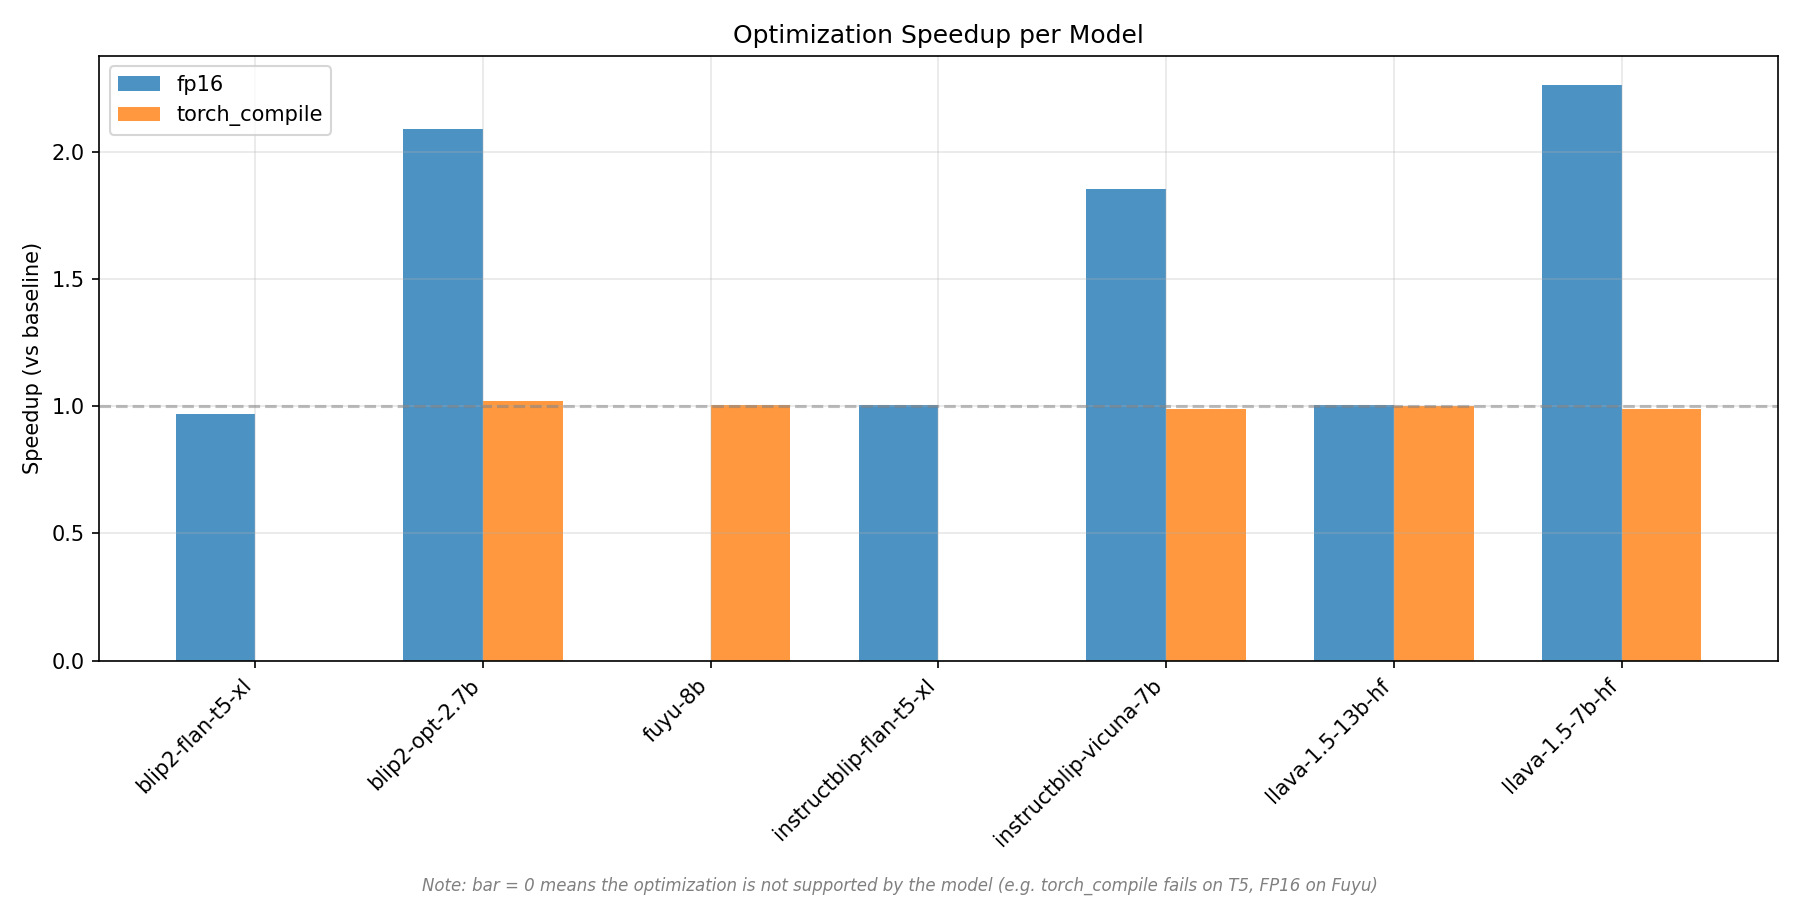
\includegraphics[width=\textwidth]{optimization_speedup.png}\\[1mm]
    \tiny FP16 helps decoder-only OPT/Vicuna/LLaMA (1.85–2.2×). \emph{Slows} T5. \texttt{torch.compile} no measurable speedup.
  \end{columns}
\end{frame}

% ====================================================================
\begin{frame}{Practical insights}
  \footnotesize
  \begin{enumerate}\setlength\itemsep{2pt}
    \item \textbf{For deployment today:} \texttt{blip2-flan-t5-xl} or \texttt{blip2-opt-2.7b}. The 7B+ tier's quality gain does not justify $\sim$15× cost.
    \item \textbf{Optimize the decoder, not the vision tower}, on every model $\geq$ 7B.
    \item \textbf{Match the optimization to generation length} via $N^*$: short answers → prefill-side (FA2, chunked prefill); long answers → decode-side (speculative, INT8/INT4, KV-cache quant).
    \item \textbf{FP16 first, attention kernels second.} Dtype flip is a 2–4× lever; FA2 inside FP16 is 1.07–1.11× at short context.
    \item \textbf{T5 is a trap with current tooling}: \texttt{torch.compile} fails, FP16 makes it slower.
    \item \textbf{Fuyu's design choice has a cost}: tokenized image patches inflate KV cache → 41 ms/token despite being 8B.
  \end{enumerate}
\end{frame}

% ====================================================================
\begin{frame}{Limitations and what's next}
  \footnotesize
  \textbf{Limitations}
  \begin{itemize}\setlength\itemsep{0pt}
    \item FLOPs for T5 backbones are estimated as $2 \times \text{params}$; calflops doesn't trace cleanly.
    \item Energy from \texttt{nvidia-smi} at 100 ms polling — a few percent, not lab-grade.
    \item No quantization (INT8/INT4) measured.
    \item FA2 evaluated only at short context; benefit at $N \gg 1k$ not captured.
  \end{itemize}
  \vspace{2mm}
  \textbf{Next steps}
  \begin{itemize}\setlength\itemsep{0pt}
    \item INT8 / GPTQ / AWQ on the 7B+ tier (decode-bound, biggest win).
    \item Speculative decoding with a small draft model.
    \item Long-context FA2 sweep (resolution 1024+, multi-image prompts).
    \item Fix the \texttt{idefics2-8b} integration.
  \end{itemize}
\end{frame}

% ====================================================================
\begin{frame}[standout]
  Thanks --- questions?\\[5mm]
  \footnotesize Repo: \texttt{github.com/smirnovlad/vlm-profiler}\\
  \footnotesize Report: \texttt{report.pdf}
\end{frame}

% ====================================================================
\appendix

\begin{frame}{Backup: per-dataset WER}
  \scriptsize
  \begin{tabular}{@{}lrrr@{}}
    \toprule
    Model & COCO Caption & ScienceQA & TextVQA \\
    \midrule
    blip2-flan-t5-xl        & 0.79 &  1.30 & 1.54 \\
    blip2-opt-2.7b          & 0.82 &  1.49 & 1.87 \\
    instructblip-flan-t5-xl & 1.85 &  1.28 & \textbf{0.86} \\
    instructblip-vicuna-7b  & \textbf{0.96} & 11.18 & 6.36 \\
    fuyu-8b                 & 4.65 &  6.42 & 7.57 \\
    llava-1.5-7b-hf         & 3.37 &  7.02 & 8.75 \\
    llava-1.5-13b-hf        & 3.36 &  7.96 & 8.06 \\
    \bottomrule
  \end{tabular}
  \vspace{2mm}

  \footnotesize
  \texttt{instructblip-vicuna-7b}: great on COCO (0.96) but breaks on ScienceQA (11.18) — likely an instruction-tuning gap on science-style prompts.
\end{frame}

\begin{frame}{Backup: parameter breakdown}
  \begin{center}
    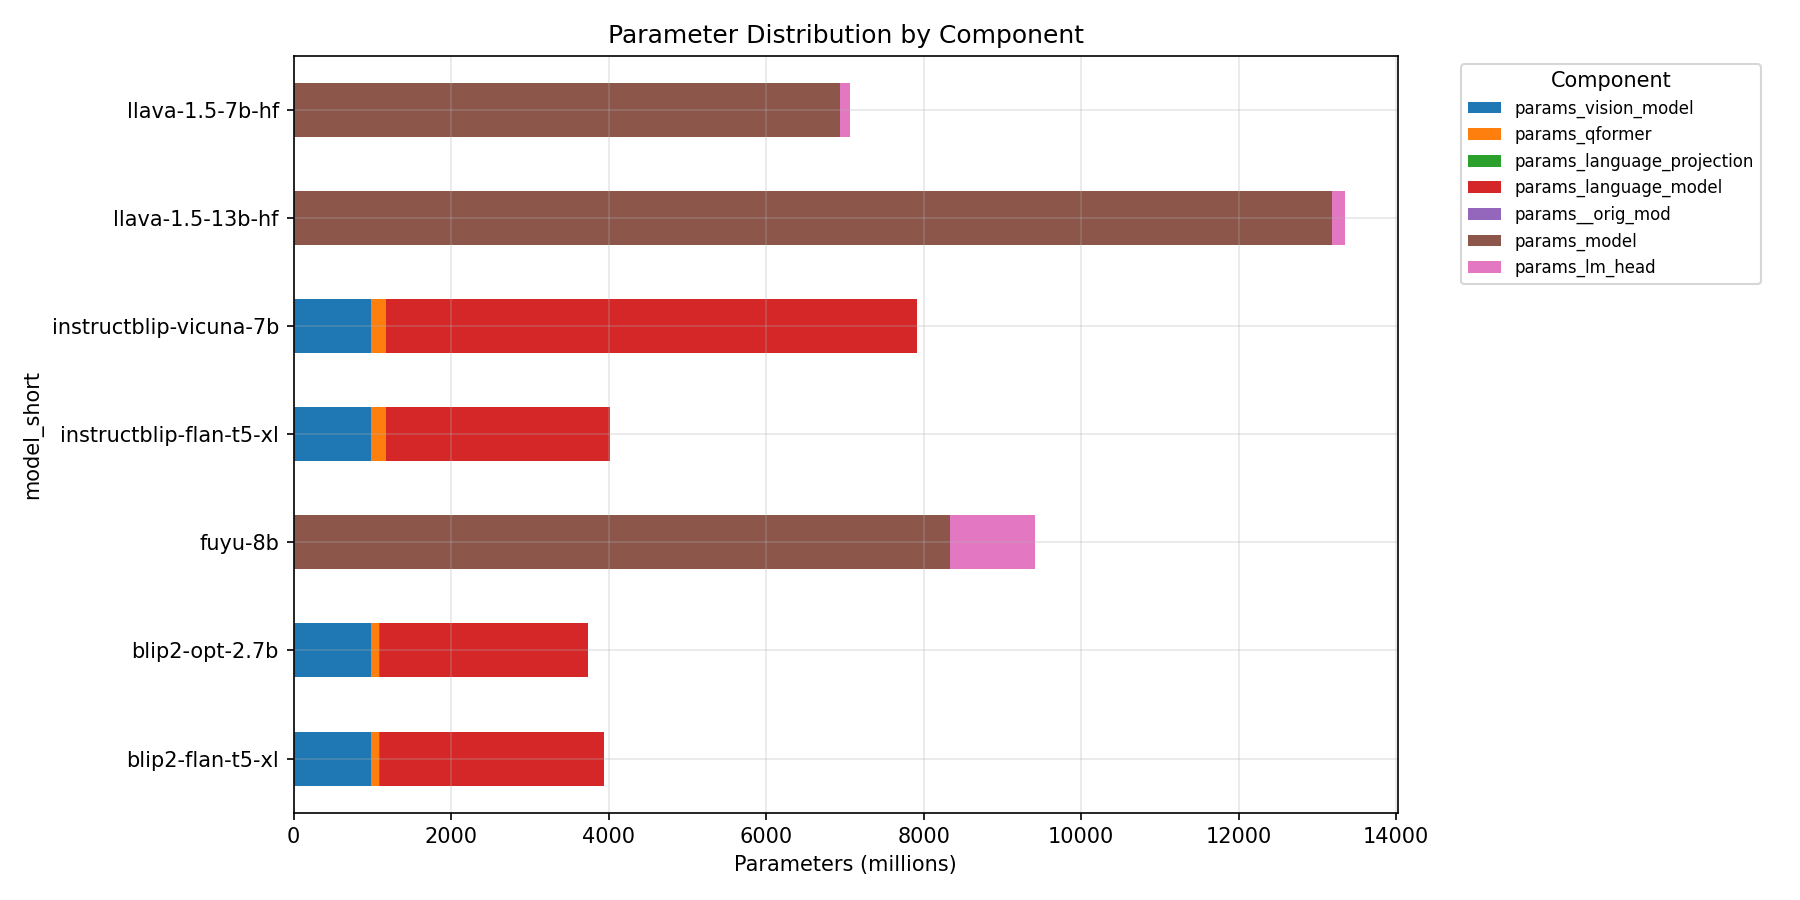
\includegraphics[width=0.78\textwidth]{param_breakdown.png}
  \end{center}
  \footnotesize
  Language decoder dominates parameter count in every model. Vision encoder $<400$ M. Matches the runtime breakdown.
\end{frame}

\begin{frame}{Backup: prefill vs.\ decode (absolute)}
  \begin{center}
    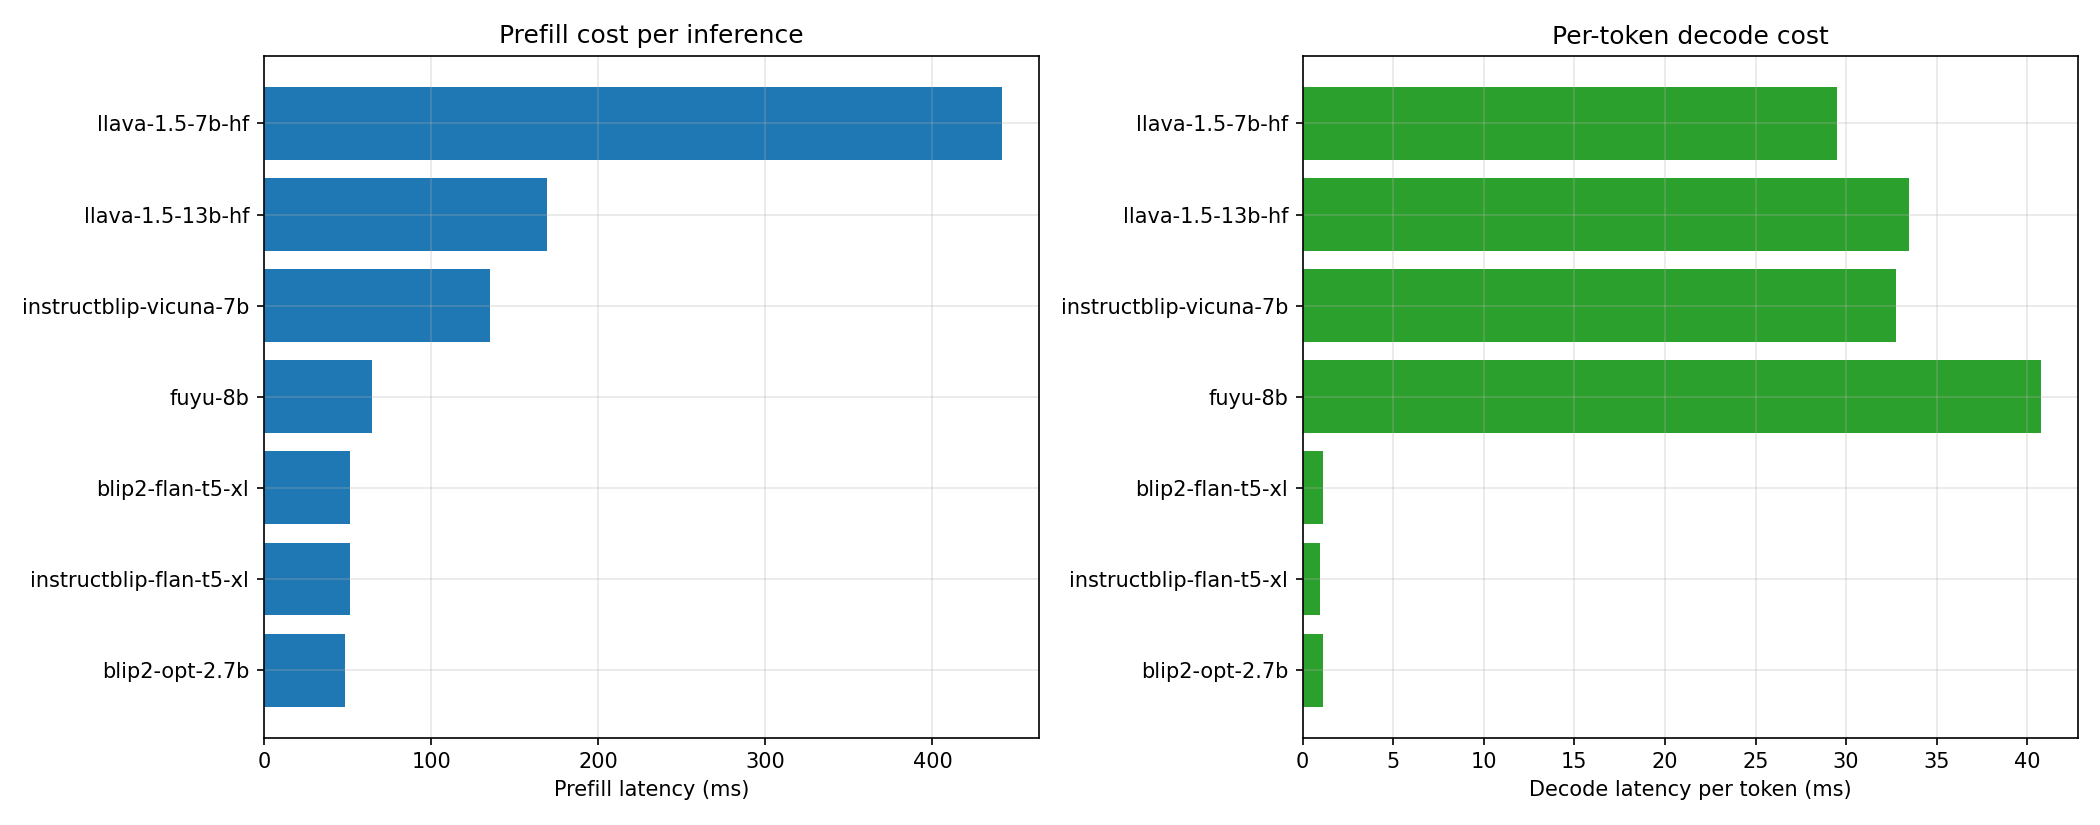
\includegraphics[width=0.85\textwidth]{prefill_vs_decode.png}
  \end{center}
  \footnotesize
  \texttt{llava-1.5-13b} is in FP16 (does not fit in 48 GiB FP32). Re-running 7B in FP16 confirms the dtype is what flips the ordering — see report Sec.\ 4.
\end{frame}

\begin{frame}{Backup: CPU vs GPU}
  \begin{center}
    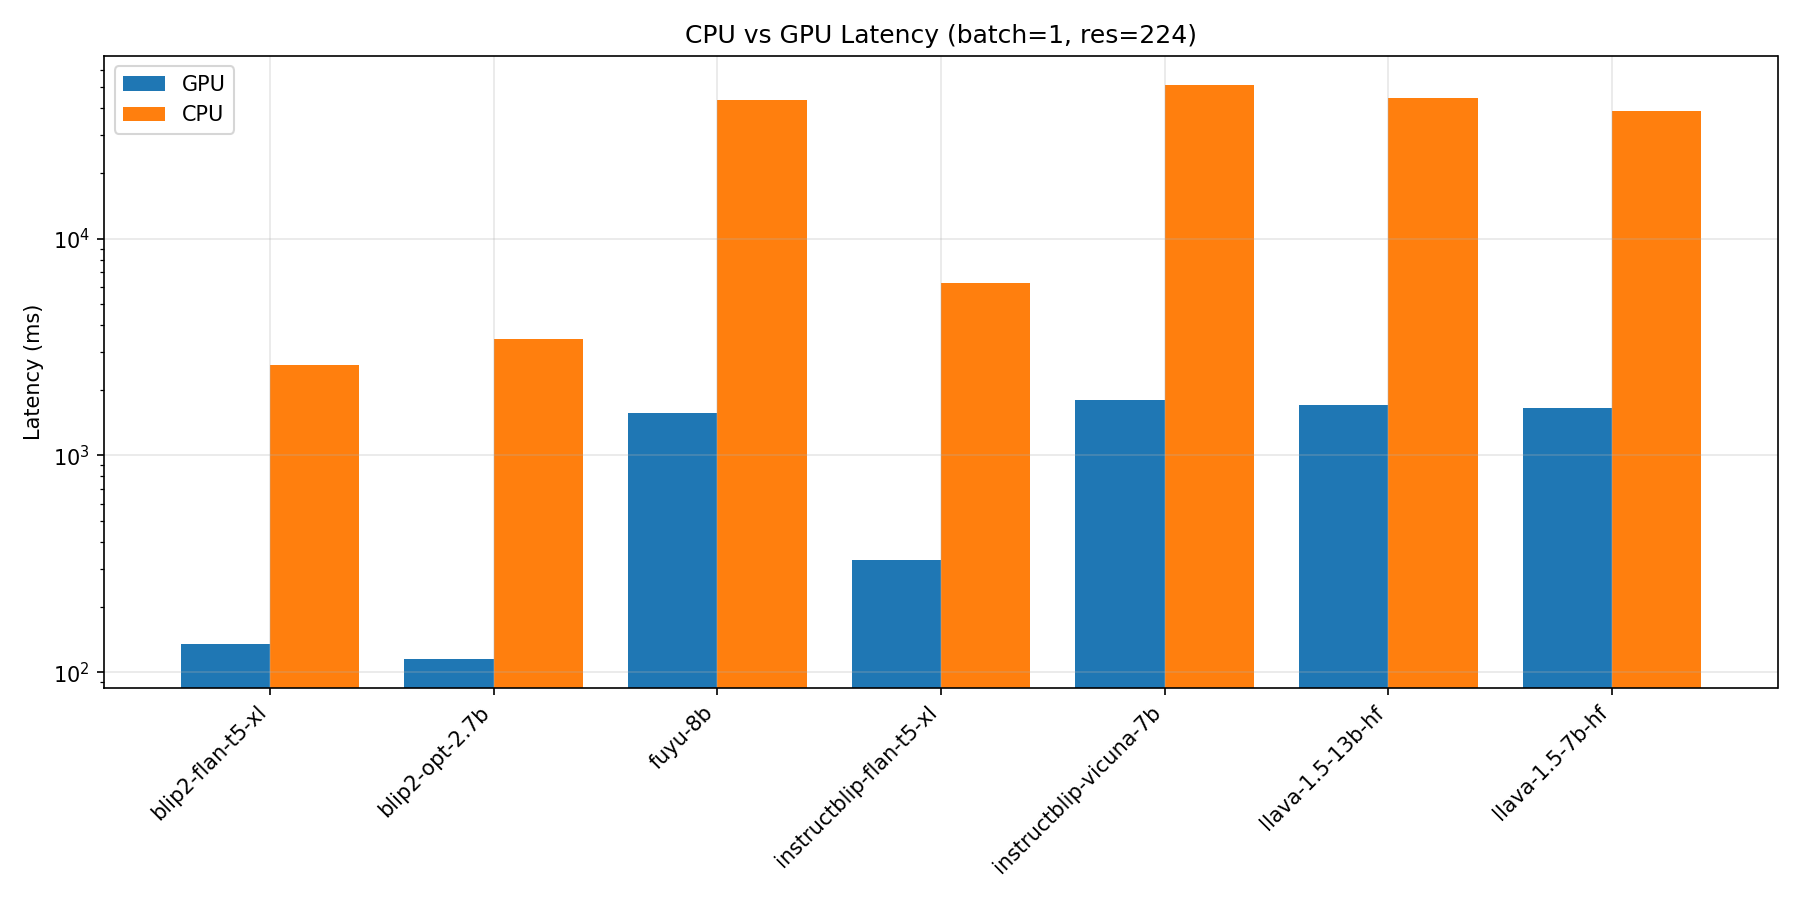
\includegraphics[width=0.85\textwidth]{cpu_vs_gpu.png}
  \end{center}
\end{frame}

\end{document}
